\chapter{Einfluss von externer Zugriffskontrolle auf die Performance in OAuth2 Systemen}
\label{sec:Einfluss von externer Zugriffskontrolle auf die Performance in OAuth2 Systemen}

Zunächst werden alle Komponenten des Systems beschrieben. Da es sich um ein OAuth2-
System handelt, gibt es alle Rollen, die auch im \autoref{subsec:OAuth2:RolleninOAuth2} beschrieben 
wurden. Also Authorization Server, Ressource Server, Client und End-Nutzer. 

\section{Keycloak als Authorization Server und Identity Provider}
\label{sec:KeycloakalsAuthorizationServerundIdentityProvider}

Keycloak ist eine Implementierung des Authorization Server der OAuth2 und OpenID 
Connect Spezifikation. Das bedeutet, dass Keycloak unter anderem dafür zuständig ist, den 
Clients Access und ID Token durch den Hybrid Flow zuzusenden. 
Keycloak wurde in der Version 12.0.4 genutzt, und in einem Docker-Container ausgeführt. 
Die genutzte Konfiguration ist in den Anlagen vorzufinden. 
Die Tokens, die Keycloak herausgibt, sind JSON Web Token und mit RSA asymmetrisch 
signiert. Konkret sind sie mit RS256 signiert, das heißt die Schlüssel sind 256 Bit groß.\smallskip

Neben einem Authorization Server ist Keycloak auch ein Identity Provider. Das 
bedeutet, dass in Keycloak Nutzer angelegt werden können und diese Nutzer auch 
verwaltet werden können. 
Damit sich Nutzer bei Keycloak authentifizieren können, musste zunächst ein Nutzer in 
Keycloak angelegt werden. Dies ist wichtig, damit dem Client überhaupt ein Token 
ausgestellt werden kann durch den Hybrid Flow. Die Charakterisierung des Nutzers ist 
an dieser Stelle wichtig, da die vorhandenen Attribute, die den Nutzern zugewiesen werden, auch 
in den Token gemappt werden und die Größe des Tokens Einfluss auf die Performance 
hat.\bigskip

\begin{figure}[htbp]
  \centering
  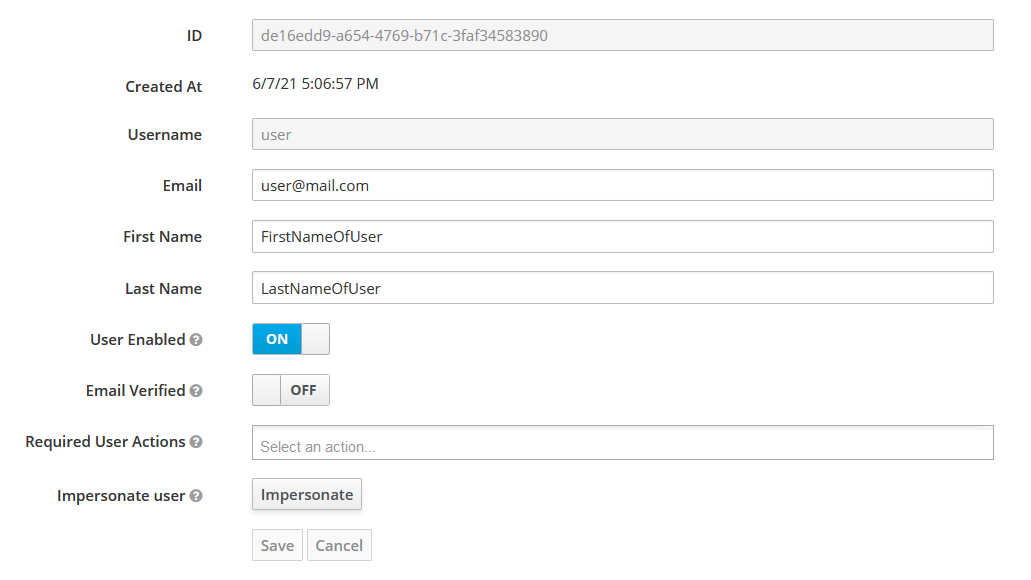
\includegraphics[width=1.0\textwidth]{gfx/keycloak-sample-user.PNG}
  \caption{Keycloak Sample User}
  \label{fig:chapter03:keycloak-sample-user}
\end{figure}

In \autoref{fig:chapter03:keycloak-sample-user} ist der erstellte Nutzer in Keycloak zu sehen. Neben 
den Standardattributen wird dem Nutzer auch eine Rolle zugewiesen, und zwar die Rolle ROLE\_USER. Dies ist in Keycloak möglich und damit lässt sich in den Applikationen eine rollenbasierte Zugriffskontrolle realisieren.\bigskip

\begin{figure}[htbp]
  \centering
  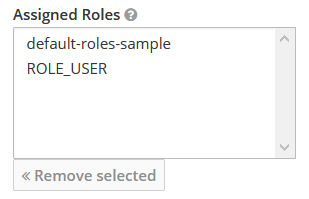
\includegraphics[width=0.5\textwidth]{gfx/keycloak-sample-user-role.PNG}
  \caption{Keycloak Sample User Role}
  \label{fig:chapter03:keycloak-sample-user-role}
\end{figure}

In \autoref{fig:chapter03:keycloak-sample-user-role} sind die zugewiesenen Rollen zu sehen. Die Rolle default-roles-sample ist eine durch Keycloak automatisch zugewiesene Rolle und hat hier keine weitere Relevanz. 
Außerdem wurde diesem Nutzer noch eine Gruppenzugehörigkeit und ein weiteres Attribut 
hinzugewiesen. Gruppenzugehörigkeiten sind in Firmen oftmals die Bürostandorte, 
Abteilungen und dergleichen. Nach Gruppenzugehörigkeiten wird in der Regel nicht 
autorisiert, denn dafür sind Rollen zuständig. Die Gruppenzugehörigkeit und das weitere 
Sample-Attribut hat hier nur den Sinn, dass es den Token umfangreicher macht und dies 
dient dazu, realistische Testbedingungen zu schaffen. Der Nutzer ist also in der Gruppe 
Users und hat als zusätzliches Attribut das statische Schlüssel-Wert-Paar Attribute1:UserAttribute1. 

\section{Erhalt eines Tokens mit Postman}
Um Token durch den Hybrid Flow zu erhalten, wird ein Client und ein Nutzer benötigt, der 
sich für den Client authentifiziert und der Authorization Server, der den Token ausstellt. 
Der erstellte Nutzer wurde im vorhergehenden Kapitel in Keycloak, dem Authorization 
Server, gezeigt. Der Nutzer muss einen Browser Agenten bedienen, damit der Client über 
den Hybrid Flow Token erhalten kann. Als Client wurde der API-Client Postman verwendet, 
der eingebauten Support für OAuth2 besitzt und mittels eines Browsers den Hybrid Flow 
ausführen und damit Postman, also der OAuth2 Client, Token erhalten kann. 

\begin{figure}[htbp]
  \centering
  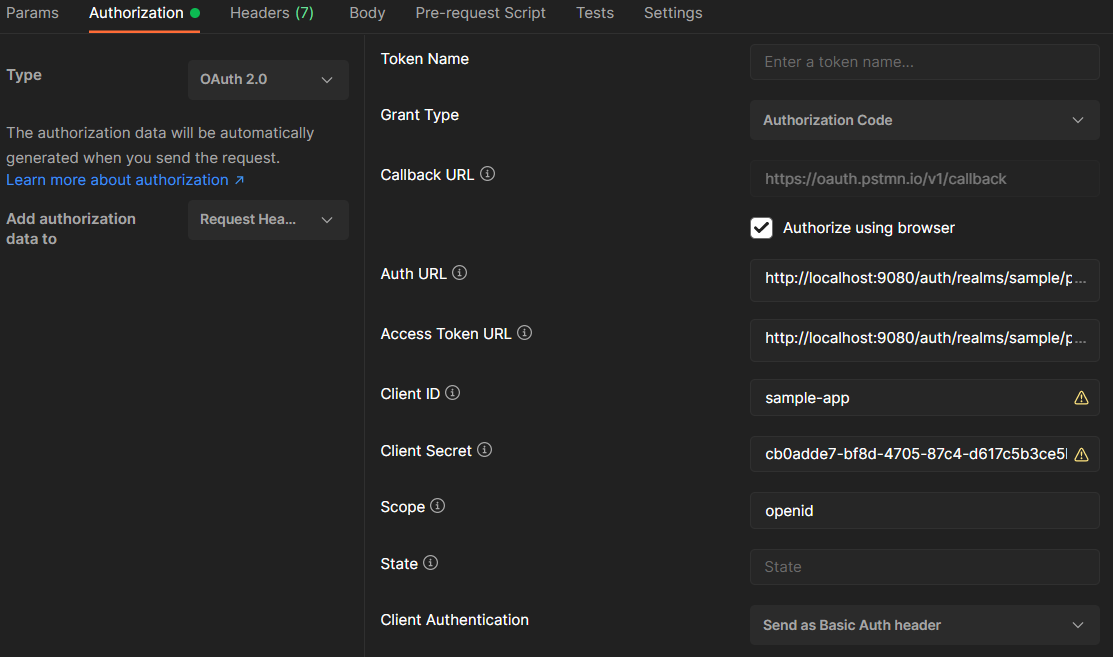
\includegraphics[width=1.0\textwidth]{gfx/postman-get-token3.PNG}
  \caption{Authorization Code Grant mit Postman}
  \label{fig:chapter03:postman-get-token3}
 \end{figure}

In \autoref{fig:chapter03:postman-get-token3} ist das Menü in Postman zu sehen. Um einen Token in Postman über den Hybrid Flow zu erhalten, müssen einige Daten eingegeben werden. 
Wie in \autoref{subsec:OAuth2:ErhaltvonToken} beschrieben, gibt es mehrere Wege wie ein Client einen Token 
erhalten kann. Hier musste als Grant Type Authorization Code angegeben werden. 
Dann musste die Auth URL, der Authorization Endpunkt des Authorization Serve, 
angeben werden. Hier wird der Browser des End-Nutzers hingeleitet, wo sich der End-Nutzer authentifizieren muss. 
Die Access Token URL ist diejenige URL, von der Postman in Austausch von einem 
Authorization Code einen Token erhalten kann. Den Authorization Code erhält Postman, 
nachdem sich der End-Nutzer bei Keycloak authentifiziert hat. 
Diese Endpunkte sind in Keycloak in der Admin-Konsole vorzufinden. 
Als Client ID und Client Secret wurden die Werte eingetragen, die bei der Registrierung des 
Clients erhalten wurden. 
Als Scope wurde openid angegeben, damit die notwendigen Nutzerattribute von dem End-Nutzer, der sich bei Keycloak authentifiziert in den ID Token gemappt werden, da diese Attribute ja benötigt werden, um eine Zugriffskontrolle zu realisieren. 
Wenn diese Anfrage in Postman abgeschickt wird, öffnet sich der Webbrowser und die Auth-URL von Keycloak wird dargestellt. Hier muss sich der End-Nutzer authentifizieren. Die Auth URL ist nachfolgend dargestellt. 

\begin{lstlisting}[language=C++,frame=tb,caption={Authorization Request},label=lst:AuthorizationRequest]
  http://localhost:9080/auth/realms/sample/protocol/openid-connect/auth?
  response_type=code
  &state=
  &client_id=sample-app
  &scope=openid
  &redirect_uri=HTTPs%3A%2F%2Foauth.pstmn.io%2Fv1%2Fcallback
\end{lstlisting}
\bigskip

In \autoref{lst:AuthorizationRequest} ist die HTTP-POST-Request dargestellt, mit der Postman, nachdem sich der End-Nutzer 
authentifiziert hat, einen Authorization Code erhält. Diesen kann Postman durch einen Token 
von Keycloak austauschen. Die Paramater, die hier an Keycloak übertragen werden, 
sind diejenigen, die auch in \autoref{subsec:OpenIDConnect:HybridFlow} beschrieben sind, nämlich:

\begin{itemize}
  \item Response\_type
  \item State
  \item Client\_Id
  \item Scope
  \item Redirect\_uri
\end{itemize}

Nachdem sich der End-Nutzer authentifiziert hat, erhält Postman einen JSON Web Token. Die 
Token-Anfrage, bei der der Authorization Code durch einen Token ausgetauscht wird, 
geschieht automatisch und wird hier nicht beschrieben.

\begin{lstlisting}[frame=tb,caption={Base64-kodierter JSON Web Token},label=lst:Base64-kodierterJSONWebToken]
  eyJhbGciOiJSUzI1NiIsInR5cCIgOiAiSldUIiwia2lkIiA6ICJhUV83TjRENmN5MEVnVnVlR2ZrSWRobG5Ud1FoYi1IVDJlM21wWWFHV0o4In0.

  eyJleHAiOjE2MjY2NDE0MzQsImlhdCI6MTYyNjYzOTYzNCwiYXV0aF90aW1lIjoxNjI2NjM5NjMzLCJqdGkiOiJiZjA3MDQwNS03NDY5LTQ1NTQtOWViOC1mNTcwMjNhMGY0ZDMiLCJpc3MiOiJodHRwOi8vbG9jYWxob3N0OjkwODAvYXV0aC9yZWFsbXMvc2FtcGxlIiwiYXVkIjoiYWNjb3VudCIsInN1YiI6ImJmNDlmODdmLTY2ZDktNDNjZS1hNzRmLTgyMzNkY2ZmODNhYiIsInR5cCI6IkJlYXJlciIsImF6cCI6InNhbXBsZS1hcHAiLCJzZXNzaW9uX3N0YXRlIjoiNzFiMzJhZjgtNTQ0OS00OTMzLWJlZmUtZDQzODAwNzdkYzI1IiwiYWNyIjoiMSIsInJlYWxtX2FjY2VzcyI6eyJyb2xlcyI6WyJkZWZhdWx0LXJvbGVzLXNhbXBsZSIsIlJPTEVfVVNFUiIsIm9mZmxpbmVfYWNjZXNzIiwidW1hX2F1dGhvcml6YXRpb24iXX0sInJlc291cmNlX2FjY2VzcyI6eyJhY2NvdW50Ijp7InJvbGVzIjpbIm1hbmFnZS1hY2NvdW50IiwibWFuYWdlLWFjY291bnQtbGlua3MiLCJ2aWV3LXByb2ZpbGUiXX19LCJzY29wZSI6Im9wZW5pZCBlbWFpbCBwcm9maWxlIiwiZW1haWxfdmVyaWZpZWQiOmZhbHNlLCJyb2xlcyI6WyJkZWZhdWx0LXJvbGVzLXNhbXBsZSIsIlJPTEVfVVNFUiIsIm9mZmxpbmVfYWNjZXNzIiwidW1hX2F1dGhvcml6YXRpb24iXSwibmFtZSI6IkZpcnN0TmFtZU9mVXNlciBMYXN0TmFtZU9mVXNlciIsImF0dHJpYnV0ZTEiOiJVc2VyQXR0cmlidXRlMSIsImdyb3VwcyI6WyIvVXNlcnMiXSwicHJlZmVycmVkX3VzZXJuYW1lIjoidXNlciIsImdpdmVuX25hbWUiOiJGaXJzdE5hbWVPZlVzZXIiLCJmYW1pbHlfbmFtZSI6Ikxhc3ROYW1lT2ZVc2VyIiwiZW1haWwiOiJ1c2VyQG1haWwuY29tIn0.

  b9BWNcf6ZaG-3sgX86YLu58vyk-HiZkDbLEdp5PgHEuZ6Q9omqjRsZCv4poQZtiqWrHSbprjiwfLadfPwz8sK9UOCrDs2KGd9Ev1nZrnI8JbhS3yfixkKTDyOOCja6KGAoYzfAnc4UVwfgP7xevBrWAnbpWGfVSStAPWBSlk0ICCHw8Kwkrly95tggsZLpuKFi7Mr0wrKlbB9-KjKYSoQhvZ6pQCFFJ83SjZ-sj_v7tkHXX79wf-exIgy2k64JBXViT66JKg9t33wnFEHtnnLG-nvoqGirPeRTZT0T_skmHNTg-p9zIxN3uYPMfKJ0o1yRUjvDD4LG1WYWKUahu82Q
\end{lstlisting}
\bigskip

In \autoref{lst:Base64-kodierterJSONWebToken} ist der Base64 kodierte Token zu sehen. Er ist in drei Teile 
unterteilt: Dem Header, dem Payload und der Signatur. Um ihn zu dekodieren und den 
Inhalt in JSON betrachten zu können, gibt es Dienste, die das Übernehmen. Auf \url{https://jwt.io/} ist es möglich, Base64 kodierte JSON Web Token zu dekodieren. 

\begin{lstlisting}[frame=tb,caption={Dekodierter JSON Web Token},label=lst:DekodierterJSONWebToken]
{
    "alg": "RS256",
    "typ": "JWT",
    "kid": "ht0BHd8h1Q_CPuOLMj2TjiBJd6ukIROuxFmimbECbsk"
}.
{
    "exp": 1626691594,
    "iat": 1626689794,
    "auth_time": 1626689528,
    "jti": "dacddb77-6de4-4464-b623-b766a8624cda",
    "iss": "http://localhost:9080/auth/realms/sample",
    "aud": "account",
    "sub": "8cf89140-e8d6-4850-b416-3cceda982ec2",
    "typ": "Bearer",
    "azp": "sample-app",
    "session_state": "c8e12b53-1203-4d8e-a27c-ea54f3f86d60",
    "acr": "0",
    "realm_access": {
      "roles": [
        "default-roles-sample",
        "ROLE_USER",
        "offline_access",
        "uma_authorization"
      ]
    },
    "resource_access": {
      "account": {
        "roles": [
          "manage-account",
          "manage-account-links",
          "view-profile"
        ]
      }
    },
    "scope": "openid email profile",
    "email_verified": false,
    "roles": [
      "default-roles-sample",
      "ROLE_USER",
      "offline_access",
      "uma_authorization"
    ],
    "name": "FirstNameOfUser LastNameOfUser",
    "attribute1": "UserAttribute1",
    "groups": [
      "/Users"
    ],
    "preferred_username": "user",
    "given_name": "FirstNameOfUser",
    "family_name": "LastNameOfUser",
    "email": "user@mail.com"
}.
[Signature]
\end{lstlisting}
\bigskip

In \autoref{lst:DekodierterJSONWebToken} ist der dekodierte JSON Web Token dargestellt, den Keycloak erstellt und an Postman gesendet hat. Wie zu sehen ist, sind die Nutzerattribute, das heißt die Standardclaims, in diesen Token gemappt. Das heißt der Vor-und-Nachname, die E-Mail-Adresse, der Nickname sowie das Claim sub. 
Zudem ist die Gruppenzugehörigkeit zu sehen, denn der Nutzer ist ja Mitglied in der Gruppe Users. Außerdem ist unter dem Schlüssel roles auch die Rolle ROLE\_USER vorzufinden. Diese Rolle wurde dem End-Nutzer in Keycloak zugewiesen und nach dieser Rolle wird bei der Schnittstelle im Ressource Server die Zugriffe kontrolliert. Das heißt in dem Token muss diese Rolle gemappt sein, ansonsten sollte kein Zugriff erlaubt werden. Die restlichen Rollen, die in diesem Token zu sehen sind wie beispielsweise default-roles-sample, wurden automatisch von Keycloak erstellt und werden hier nicht weiter erläutert.\smallskip

Außerdem sind die Claims vorzufinden, die in einem ID Token Pflicht sind wie beispielsweise exp, der angibt, wann der Token abläuft. Erklärungen zu diesen Claims sind in \autoref{subsec:OpenIDConnect:IDToken} zu finden. Diese werden hier nicht weiter erläutert. 
Im Header ist unter anderem das Claim alg: RS256 vorzufinden, das angibt, dass der Token durch RSA mit 256 Bit großen Schlüssel asymmetrisch signiert ist. Der Ressource Sever kann sich den passenden öffentlichen Schlüssel von Keycloak über den JSON Web Key Set Endpunkt holen und damit die Authentizität und Integrität des Tokens validieren. 
Nun wurde also durch den Authorization Code Grant ein Token von dem Authorization Server Keycloak erhalten mit dem es möglich ist, auf die HTTP-Schnittstellen eines Ressource Servers zuzugreifen. Diese Ressource Server werden im nachfolgenden Kapitel beschrieben. 

\section{Ressource Server}
Beide Ressource Server sind in Java mithilfe des Spring-Frameworks implementiert. Die Ressource Server sind Spring-Boot Anwendungen, das bedeutet, dass ein Apache Tomcat Webserver in der Applikation eingebettet ist und automatisch gestartet wird. Die Ressource Server können somit HTTP-Anfragen von Clients entgegennehmen und diese beantworten.\smallskip

Die verwendete Spring-Boot Version ist 2.4.8 mit Apache Tomcat 9.0.48, welcher über den Port 8080 erreichbar ist. Alle Versionen der verwendeten Technologien wie die Datenbank und der Object-Relational Mapper Hibernate können aus der Spring-Boot Version hergeleitet werden und werden deshalb im weiteren Verlauf nicht genannt. Als Java Runtime Environment (JRE) wurde Version 11 verwendet.\smallskip

Gemäß der OAuth2 Spezifikation bezeichnet man diese Server Ressource Server, weil sie valide Tokens erwarten, die von einem Authorization Server ausgestellt werden, damit sie den Clients Zugriff auf ihre Schnittstellen geben können. Im weiteren Verlauf werden beide Ressource Server auf ihre Performance getestet. Der einzige Unterschied zwischen beiden Servern besteht darin, wie sie Zugriffsentscheidungen evaluieren, das heißt wie sie ermitteln, ob der Client berechtigt ist auf die Schnittstelle des Servers zuzugreifen. Dies wird als Zugriffskontrolle bezeichnet. Der eine Ressource Server implementiert diese Zugriffskontrolle in der Spring-Boot Applikation selbst, während der andere diese entkoppelt mit Open Policy Agent, das ein externes Programm ist. Es ist per HTTP für den Server erreichbar ist, um eine Zugriffsentscheidung zu erhalten.\smallskip

Zu erwähnen ist, dass eine Implementierung von Ressource Servern grundsätzlich in jeder Programmiersprache erfolgen kann, die HTTP-, JSON-, Base64-Kodierung-sowie-RSA unterstützt. 

\subsection{Schnittstelle}
\label{subsec:Schnittstelle}
Beide Ressource Server haben eine HTTP-GET-Schnittstelle implementiert, welche Daten aus einer SQL-Datenbank holt und sie dem anfragenden Client sendet. Dies ist genau die Schnittstelle, die nicht für alle frei zugänglich ist, sondern nur Nutzern zur Verfügung steht, die einen validen JSON Web Token haben und der Rolle ROLE\_USER zugehörig sind. 

\begin{lstlisting}[language=Java,frame=tb,caption={HTTP-Schnittstelle der Ressource Server},label=lst:HTTP-Schnittstelleder Server]
  /**
  * {@code GET  /documents} : get all the documents.
  *
  * @return the {@link ResponseEntity} with status {@code 200 (OK)} 
  * and the list of documents in body.
  */
  @GetMapping("/documents")
  public List<Document> getAllDocuments() {
     log.debug("REST request to get all Documents");
     return documentService.findAll();
  }
\end{lstlisting}
\bigskip

In \autoref{lst:HTTP-Schnittstelleder Server} ist diese Schnittstelle dargestellt. Sie wird auf „/documents“ gemappt, das bedeutet, dass falls der Ressource Server auf dem localhost gestartet wird, und der Client sich ebenso auf dem localhost befindet, er diese Schnittstelle über den Pfad „localhost:8080/documents“ ansprechen kann. 8080 ist hierbei der Port, auf dem Apache Tomcat HTTP-Anfragen abhört.
Diese Schnittstelle wurde in eine für Spring-Anwendungen typischen objektorientierten Architektur implementiert.

\begin{figure}[htbp]
  \centering
  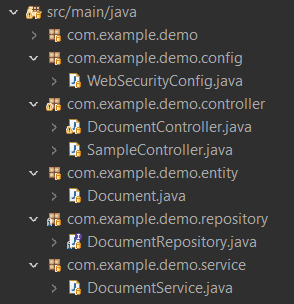
\includegraphics[width=0.5\textwidth]{gfx/projekstruktur-spring.png}
  \caption{Projekstruktur Spring Applikation}
  \label{fig:chapter03:projekstruktur-spring}
\end{figure}
\bigskip

In \autoref{fig:chapter03:projekstruktur-spring} ist die Projektstruktur dargestellt und die typische in Spring-Anwendungen vorzufindende geschichtete Architektur. Es gibt die Packages *.config, *.controller, *.entity, *.repository und *.service.\smallskip

In dem *.controller-Package befindet sich die DocumentController-Klasse, die in Abbildung 13 zu sehen ist. Diese ruft eine Funktion der DocumentService-Klasse aus dem *.service-Package auf, welche alle Daten aus dem DocumentRepository in dem Package *.repository abruft. Dieses Repository ist ein JPARepository. JPA steht für Jakarta Persistence API, welche eine Spezifikation für die Schnittstelle zwischen Java-Anwendungen und SQL-Datenbanken ist. Als Implementierung dieser Spezifikation wird in dem Projekt der object-relational Mapper (ORM) Hibernate verwendet. 
Das JPARepository implementiert unter anderem die Funktion .findAll(), welche alle Daten aus der Document-Table aus der verbundenen SQL-Datenbank holt. Diese Funktion wird in der DocumentService-Klasse aufgerufen.
In dem Package *.entity befindet sich die Klasse Document, welche die durch Hibernate annotierte Entität darstellt. Diese repräsentiert die Table Document in der SQL-Datenbank. 
Als Datenbank wird H2 Database Engine verwendet. Sample-Daten werden in diese Datenbank bei dem Start der Anwendung automatisch durch das SQL-insert-Skript geladen. Dieses Skript ist in dem Projekt unter src/main/resources/data.sql zu finden. 
Diese HTTP-GET-Schnittstelle /documents sendet autorisierten anfragenden Clients alle Document-Daten in JSON aus der SQL-Datenbank zu. Das eine SQL-Datenbank mit der Applikation verbunden wurde, dient der Simulierung von realistischen Testbedingungen, da in der Regel HTTP-GET-Schnittstellen Daten aus einer Datenbank holen und sie den anfragenden Clients zusenden. Zudem wurde keine Cache Konfiguration von Hibernate verwendet, damit jede Anfrage von Clients gleichbehandelt wird und keine Inkonsistenzen bei den Latenzen entstehen. 

\subsection{Spring Security OAuth2}
Um die Server und die Schnittstelle als OAuth2 Ressource Server zu konfigurieren, wurde Spring Security verwendet, welches ein Teilprojekt des Spring Frameworks ist. 
Um Zugriffe auf Schnittstellen nur Anfragen, die einen validen JSON Web Token haben zu erlauben, implementiert Spring Security eine SecurityFilterChain. Diese ist eine Implementierung der Servlet Filter Spezifikation. 

\begin{figure}[htbp]
  \centering
  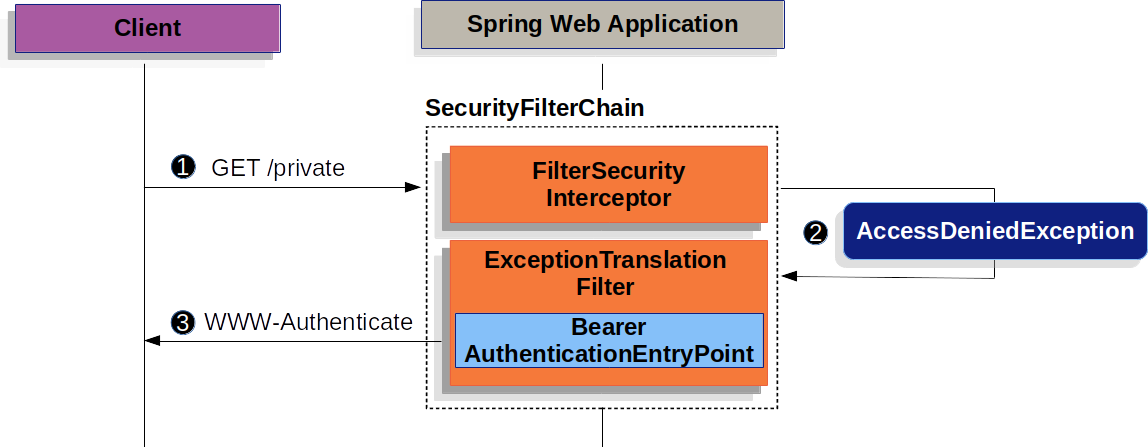
\includegraphics[width=1.0\textwidth]{gfx/bearerauthenticationentrypoint.png}
  \caption{Bearer Token Authentication \citep{springsecuritydoc:2021}}
  \label{fig:chapter03:bearerauthenticationentrypoint}
\end{figure}
\bigskip

In \autoref{fig:chapter03:bearerauthenticationentrypoint} ist die Funktionsweise der SecurityFilterChain abgebildet. Der Client sendet eine Anfrage auf den durch OAuth2 geschützten Pfad /private der Spring Web Application. Falls die Anfrage nicht beantwortet werden darf, weil der Token des Clients invalide oder überhaupt kein Token vorhanden ist, wird eine AccessDeniedException geworfen und der Client wird aufgefordert sich zu authentifizieren. Ein valider Token, den der Client an den Server sendet, entspricht konzeptionell einer Authentifikation. 
Damit die Ressource Server die Tokens validieren können, musste der JSON Web Key Set Endpunkt des Authorization Server in der Spring-Boot-Applikation angegeben werden. Dadurch kann die Applikation sich die öffentlichen Schlüssel der RSA-Signatur von diesem Endpunkt holen und damit die RSA-Signatur validieren, indem aus dem durch Base64 kodierten Header und Payload des JSON Web Tokens die Signatur berechnet und auf Gleichheit überprüft wird. Da der Ressource Server auf derselben Host-Maschine wie Keycloak, der Authorization Server, läuft, ist der Endpunkt in diesem Fall:

\begin{lstlisting}
  http://localhost:9080/auth/realms/sample/protocol/openid-connect/certs
\end{lstlisting}
\smallskip

Zudem werden die folgenden Claims des JSON Web Tokens validiert:

\begin{description}
  \item[exp:] Der exp-Claim (Expiration Time) ist derjenige Claim der angibt, bis wann der Token gültig ist.
  \item[nbf:] Der nbf-Claim (Not Before) gibt den Zeitpunkt an, ab wann der Token akzeptiert werden darf.
  \item[iss:] Der iss-Claim (Issuer) gibt die \ac{URI} des Authorization Server an. Sie sollte dem Authorization Server entsprechen, von dem auch die öffentlichen Schlüssel für die RSA-Signatur geholt werden. 
\end{description}

In beiden Ressource Servern wird eine erfolgreiche Authentifizierung, ein valider JSON Web Token, der von Keycloak erstellt wurde, erwartet. Die Autorisierung aber, das heißt die Prüfung, ob der authentifizierte Nutzer die benötigten Rechte verfügt, um Zugriff auf die Schnittstelle zu erhalten, wird in den zwei Ressource Servern auf zwei unterschiedliche Weisen realisiert und in den nachfolgenden zwei Kapiteln beschrieben.

\subsection{Spring Security Ressource Server mit interner Zugriffskontrolle}

Um eine rollenbasierter Zugriffskontrolle in dem Ressource Server selbst zu realisieren, wurde JwtAuthenticationConverter verwendet, das Teil von Spring Security ist.

\begin{figure}[htbp]
  \centering
  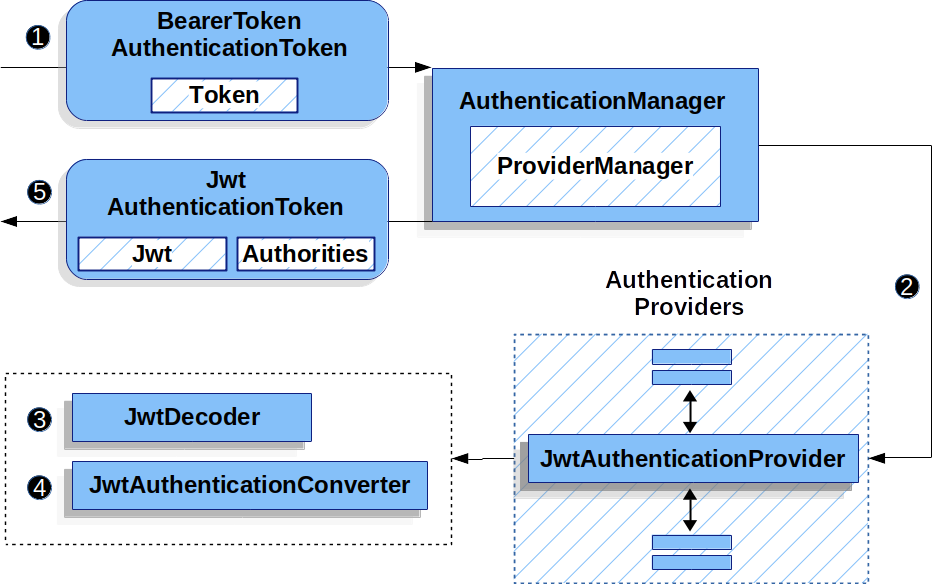
\includegraphics[width=1.0\textwidth]{gfx/jwtauthenticationprovider.png}
  \caption{JWT Authentication Provider \citep{springsecuritydoc:2021}}
  \label{fig:chapter03:jwtauthenticationprovider}
\end{figure}
\bigskip

In \autoref{fig:chapter03:jwtauthenticationprovider} ist der Ablauf dargestellt, um eine rollenbasierte Zugriffskontrolle in dem Server, also der Spring-Boot Applikation, mit dem JwtAuthenticationConverter zu realisieren. Im Wesentlichen wird hier der JSON Web Token durch den JWTAuthenticationProvider von einem JwtDecoder dekodiert, verifiziert und validiert und von dem JwtAuthenticationConverter werden Autoritäten in eine Collection gemappt. Als JwtDecoder wird die Nimbus Bibliothek verwendet \citep{springsecuritydoc:2021}.
Der JwtAuthenticationConverter wurde so konfiguriert, dass er Rollen aus dem JSON Web Token in sogenannte GrantedAuthorities mappt. Diese sind Objekte, die Privilegien von Nutzern widerspiegeln wie beispielsweise Rollen \citep{springsecuritydoc:2021}. 

\begin{lstlisting}[language=Java,frame=tb,caption={JwtAuthenticationConverter},label=lst:JwtAuthenticationConverter]
  @Bean
  public JwtAuthenticationConverter jwtAuthenticationConverter() {
      JwtGrantedAuthoritiesConverter grantedAuthoritiesConverter 
          = new JwtGrantedAuthoritiesConverter();
      grantedAuthoritiesConverter.setAuthoritiesClaimName("roles");
      grantedAuthoritiesConverter.setAuthorityPrefix("");        
  
      JwtAuthenticationConverter jwtAuthenticationConverter 
          = new JwtAuthenticationConverter();
      jwtAuthenticationConverter.
          setJwtGrantedAuthoritiesConverter(grantedAuthoritiesConverter);
      return jwtAuthenticationConverter;
  }    
\end{lstlisting}
\bigskip

In \autoref{lst:JwtAuthenticationConverter} ist die verwendete Konfiguration dargestellt. Es wird in dem JSON Web Token, der von dem Client gesendet wurde, nach dem Claim roles in dem Payload des Tokens gesucht und die Werte, die darin enthalten sind in GrantedAuthorities konvertiert. In dem Claim roles steht unter anderem auch die Rolle des Nutzers, der sich bei Keycloak authentifiziert hat, und zwar ROLE\_USER. Siehe Abbildung 13 Keycloak Access Token.
Um die Schnittstelle aus \autoref{subsec:Schnittstelle} nur Nutzern zugänglich zu machen, die die Autorität ROLE\_USER besitzen, wurde HTTPSecurity verwendet, das Teil von Spring Security ist. 

\begin{lstlisting}[language=Java,frame=tb,caption={HTTPSecurity},label=lst:HTTPSecurity]
  @Override
  protected void configure(HTTPSecurity HTTP) throws Exception {
      HTTP
          .authorizeRequests(authorize -> authorize
              .mvcMatchers("/documents").hasAuthority("ROLE_USER")
              .anyRequest().permitAll()
          )   
          .oauth2ResourceServer(OAuth2ResourceServerConfigurer::jwt);
  } 
\end{lstlisting}
\bigskip

In \autoref{lst:HTTPSecurity} ist die verwendete Konfiguration zu sehen. Hierbei wurde konfiguriert, dass auf den Pfad /documents nur zugegriffen werden darf, wenn dem anfragenden Client die GrantedAuthority ROLE\_USER zugewiesen wurde. 

\subsection{Spring Security Ressource Server mit externer Zugriffskontrolle}
Um die Zugriffskontrolle von dem zweiten Ressource Server zu entkoppeln, wurde der AccessDecisionManager verwendet, der Teil von Spring Security ist und es erlaubt Zugriffsentscheidungen externen Programmen zu überlassen. 
Als externes Programm um diese Zugriffsentscheidungen zu fällen, wurde Open Policy Agent in der Version 0.30.2 verwendet, das in einem Docker-Container ausgeführt wird und auf dem gleichen Host wie der Ressource Server läuft. 

\subsubsection{Rollenbasierte Zugriffskontrolle mit Open Policy Agent}
Zunächst wird die Systemarchitektur dargestellt, die das Zusammenspiel zwischen dem Authorization Server, Keycloak, dem Ressource Server, der Spring-Boot Applikation und dem Open Policy Agent erklärt. 

\begin{figure}[t]
  \centering
  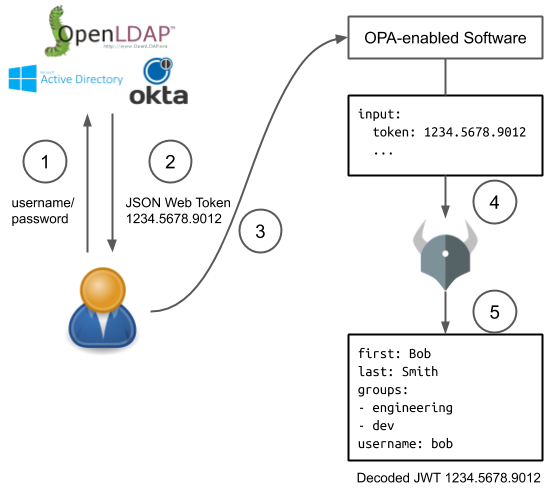
\includegraphics[width=0.8\textwidth]{gfx/data-jwt.png}
  \caption{Open Policy Agent und OAuth2 \citep{opaexternaldata:2021}}
  \label{fig:chapter03:data-jwt}
\end{figure}
\bigskip

In \autoref{fig:chapter03:data-jwt} ist die Systemarchitektur dargestellt. Zunächst authentifiziert sich der End-Nutzer bei dem Authorization Server. Hier ist als Beispiel Okta dargestellt, in diesem System wird allerdings Keycloak verwendet. Nachdem sich der End-Nutzer authentifiziert hat, erhält der Client einen JSON Web Token.
Mit diesem JSON Web Token sendet der Client eine Anfrage an die OPA-enabled Software. Dies ist der Ressource Server, also die Spring-Boot Applikation. 
Um eine Zugriffsentscheidung zu evaluieren, muss die OPA-enabled Software nun die angefragte Schnittstelle inklusive Input-Daten an Open Policy Agent senden. Diese Input-Daten sind die JSON Web Token, in welchem unter anderem auch Nutzerattribute vorhanden sind, anhand dessen Open Police Agent mithilfe programmierter Zugriffsrichtlinien in Rego, eine Zugriffsentscheidung trifft und diese der OPA-enabled Software mitteilt, woraufhin der Client eine Antwort auf seine Anfrage erhält basierend auf der Zugriffsentscheidung von Open Policy Agent. 

\begin{lstlisting}[frame=b,caption={Rollenbasierte Zugriffsrichtlinie in Rego},label=lst:RollenbasierteZugriffsrichtlinieinRego]
  package HTTP.authz

  default allow = false
  
  allow {
      input.method == "GET"
      input.path == ["documents"]
      token.payload.roles[_] == "ROLE_USER"
  }
  
  allow {
      input.method == "GET"
      input.path == ["h2-console"]
  }
  
  # Helper to get the token payload.
  token = {"payload": payload} {
      [header, payload, signature] := io.jwt.decode(input.auth.token.tokenValue)  
  }
\end{lstlisting}
\bigskip

In \autoref{lst:RollenbasierteZugriffsrichtlinieinRego} ist die verwendete programmierte rollenbasierte Zugriffskontrolle in Rego, der Programmiersprache von Open Policy Agent, um Zugriffsrichtlinien zu definieren, dargestellt. 
Es wird zunächst der JSON Web Token, den Open Policy Agent von dem Ressource Server erhält, dekodiert, da JSON Web Token in Base64 kodiert sind. Neben dem Token wird Open Policy Agent auch die angefragte HTTP-Schnittstelle mitgeteilt. 
In der ersten allow Methode, wird definiert, dass auf eine GET-Anfrage auf den Pfad documents, nur Zugriff erhalten werden darf, falls in dem Payload des JSON Web Token der Claim roles vorhanden ist und in diesem Claim der Wert ROLE\_USER vorhanden ist. Falls dem so ist, wird dem Ressource Server mitgeteilt, dass der Client autorisiert ist, eine Antwort auf seine Anfrage zu erhalten. 
Die zweite allow-Methode wird hier nicht weiter erläutert. Anfragen, die nicht der Schnittstelle documents oder h2-console entsprechen, werden grundsätzlich abgelehnt. 

\subsubsection{Spring Security AccessDecisionManager}
Um dem Ressource Server, Open Policy Agent die Zugriffsentscheidungen zu überlassen, wurde der AccessDecisionManager verwendet, der Teil von Spring Security ist. 

\begin{figure}[htbp]
  \centering
  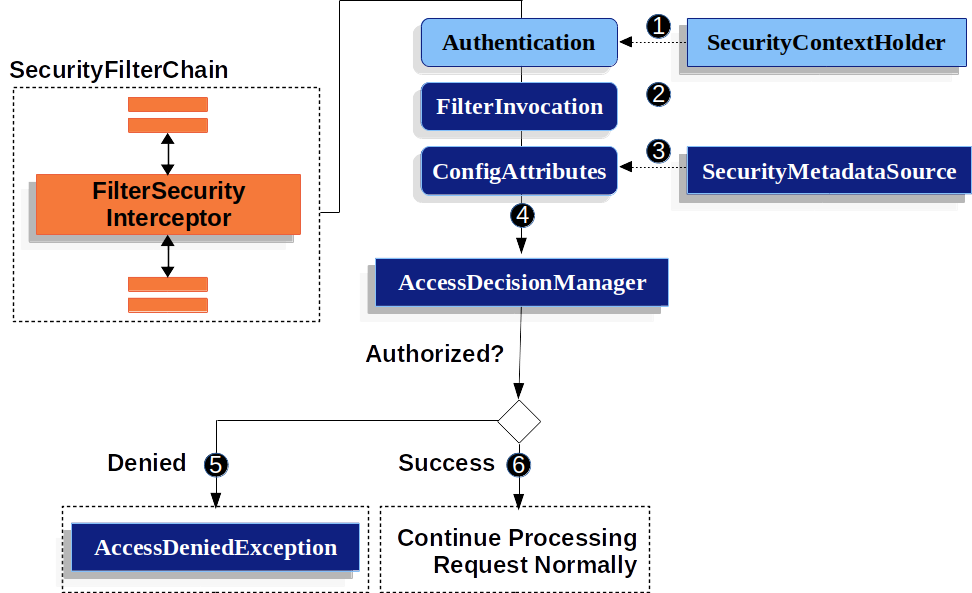
\includegraphics[width=0.8\textwidth]{gfx/filtersecurityinterceptor.png}
  \caption{AccessDecisionManager in Spring Security \citep{springsecuritydoc:2021}}
  \label{fig:chapter03:filtersecurityinterceptor}
\end{figure}
\bigskip

In \autoref{fig:chapter03:filtersecurityinterceptor} ist die Funktionsweise des AccessDecisionManagers dargestellt. Zunächst durchläuft die ankommende Anfrage des Clients die SecurityFilterChain. Im Fall einer erfolgreichen Authentifikation, was im Falle von OAuth2 einer erfolgreichen Validierung des JSON Web Tokens entspricht, trifft der AccessDecisionManager eine Zugriffsentscheidung. 
In dem AccessDecisionManager-Objekt wurde die Funktion vote() implementiert, die eine HTTP-Verbindung mit dem Open Policy Agent aufbaut, der auf der gleichen Host-Maschine wie die Spring-Boot Applikation läuft, um eine möglichst geringe Latenz zwischen beiden Programmen zu haben. Dies würde in den allermeisten Anwendungsszenarien auch im Produktiveinsatz so gemacht werden, da Open Policy Agent äußerst leichtgewichtig ist in der Belegung des Arbeitsspeichers. Die vote()-Funktion, sendet Open Policy Agent alle nötigen Informationen, damit dieser anhand dieser Informationen mit der programmierten Zugriffsrichtlinie eine Zugriffsentscheidung treffen kann, also:

\begin{itemize}
  \item Der Pfad auf den der Client zugreifen möchte
  \item Die HTTP-Methode, mit der der Client auf diesen Pfad zugreifen möchte (GET, PUT, POST etc.)
  \item Die Input-Daten, also der in Base64-kodierte JSON Web Token, welcher in dem SecurityContextHolder-Objekt gespeichert wird
\end{itemize}

Daraufhin wird dem Ressource Server von Open Policy Agent, eine Zugriffsentscheidung per HTTP mitgeteilt. Anhand dieser Entscheidung erlaubt oder verweigert der Ressource Server dem Client den Zugriff auf die Schnittstelle. 
Es wurde nun beide Ressource Server mit ihrer jeweiligen Zugriffskontrolle beschrieben. 

\section{Performancetests mit Apache JMeter}
Um Performancetests auf beiden Ressource Server durchzuführen und die Ergebnisse vergleichend auszuwerten, um den Einfluss von externer Zugriffskontrolle mit Open Policy Agent auf OAuth2 Ressource Server zu untersuchen, wurde Apache JMeter in der Version 5.4.1 verwendet. Mit Apache JMeter ist es möglich durch die Verwendung von Threads, Nutzer zu simulieren, die HTTP-Anfragen an einen Server senden. In diesen HTTP-Anfragen wird jeweils ein valider JSON Web Token an die Ressource Server gesendet und diese evaluieren jeweils eine Zugriffsentscheidung. Es wird gemessen, wie lange die Ressource Server jeweils für eine Evaluierung einer Zugriffsentscheidung und das darauffolgende Senden der Antwort benötigen.\smallskip

Wenn ein Single Sign-On mittels OpenID Connect implementiert wird, senden eingeloggte Nutzer bei jeder Anfrage den JSON Web Token, den sie nach der Authentifikation von dem Authorization Server erhalten haben an den Ressource Server, um Zugriff auf dessen Schnittstellen zu erhalten. Bei diesen Performancetests werden eingeloggte Nutzer simuliert, die auf Schnittstellen eines Servers zugreifen möchten. Jeder Thread entspricht einem eingeloggten Nutzer.\smallskip

Es wurden drei Testpläne erstellt, die verschiedene Aspekte der Server testen, wobei alle drei unter dem Überpunkt der Performance gehören. Die drei Testpläne werden als Lasttest, Skarlierbarkeitstest und Stresstest bezeichnet. 

\begin{description}
  \item[Lasttest:] Bei dem Lasttest wird der Server mit üblicher Last getestet und die Latenz gemessen. 
  \item[Skalierbarkeitstest:] Bei dem Skalierbarkeitstest wird ansteigende Last auf dem Server generiert, wobei hierbei untersucht werden soll, inwiefern sich Antwortzeiten des Servers bei hinzukommender Last ändern. 
  \item[Stresstest:] Bei dem Stresstest wird eine unüblich hohe Last auf den Server generiert, um die Grenzen des Servers feststellen zu können. 
\end{description}

Bei jedem Test wird auch die \ac{CPU}-Auslastung und Arbeitsspeicherbelegung betrachtet. Alle Tests wurden verteilt gestartet, das bedeutet, dass Client (Apache JMeter) und Server auf jeweils einem Rechner laufen. Dies dient dem Zweck, dass die Testergebnisse nicht verfälscht werden, da bei einer hohen Anzahl von Threads sowohl das Senden von HTTP-Anfragen CPU-Last erzeugt als auch das Abarbeiten der Anfragen durch den Server und beide Prozesse sich gegenseitig nicht ausbremsen sollten. Die verwendete Systemhardware von Client und Server, ist in \autoref{subsec:SystemhardwareundTestumfeld} zu sehen.

\subsection{Lasttest}
In dem Lasttest wurde eine übliche Last auf den Server generiert und mittels sogenannten Listener die Ergebnisse gemessen und protokolliert. 

\begin{figure}[htbp]
  \centering
  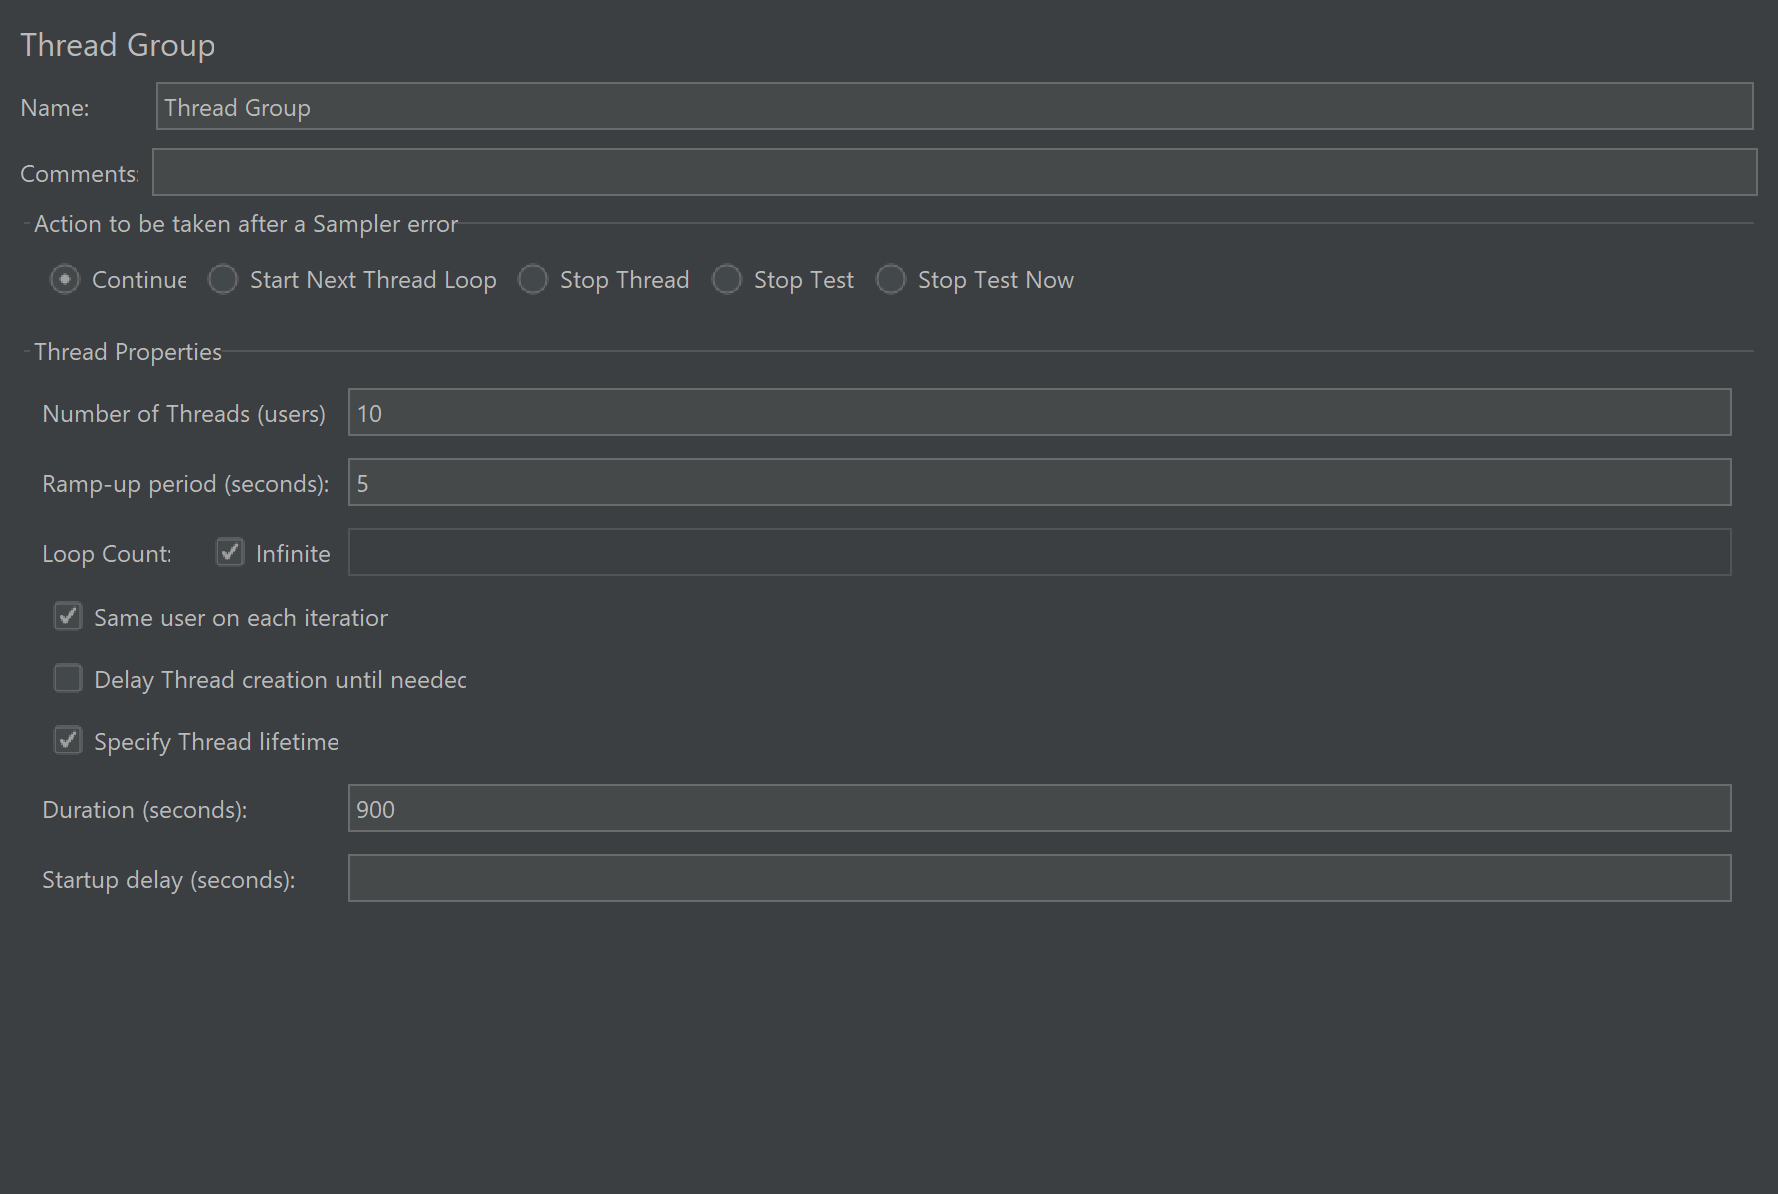
\includegraphics[width=1.0\textwidth]{gfx/Thread Group-Last.png}
  \caption{Thread Group-Last}
  \label{fig:chapter03:ThreadGroup-Last}
\end{figure}
\bigskip

In \autoref{fig:chapter03:ThreadGroup-Last} ist die verwendete Konfiguration dargestellt. Es werden zehn Threads gestartet, die jeweils gleichzeitig HTTP-Anfragen an den Server senden. Als Ramp-up period wurde fünf Sekunden gesetzt. Das bedeutet, es dauert fünf Sekunden, bis alle zehn Threads gestartet sind. Als Duration ist 900 Sekunden eingestellt worden, das bedeutet das der Test 15 Minuten dauert. 

\begin{figure}[htbp]
  \centering
  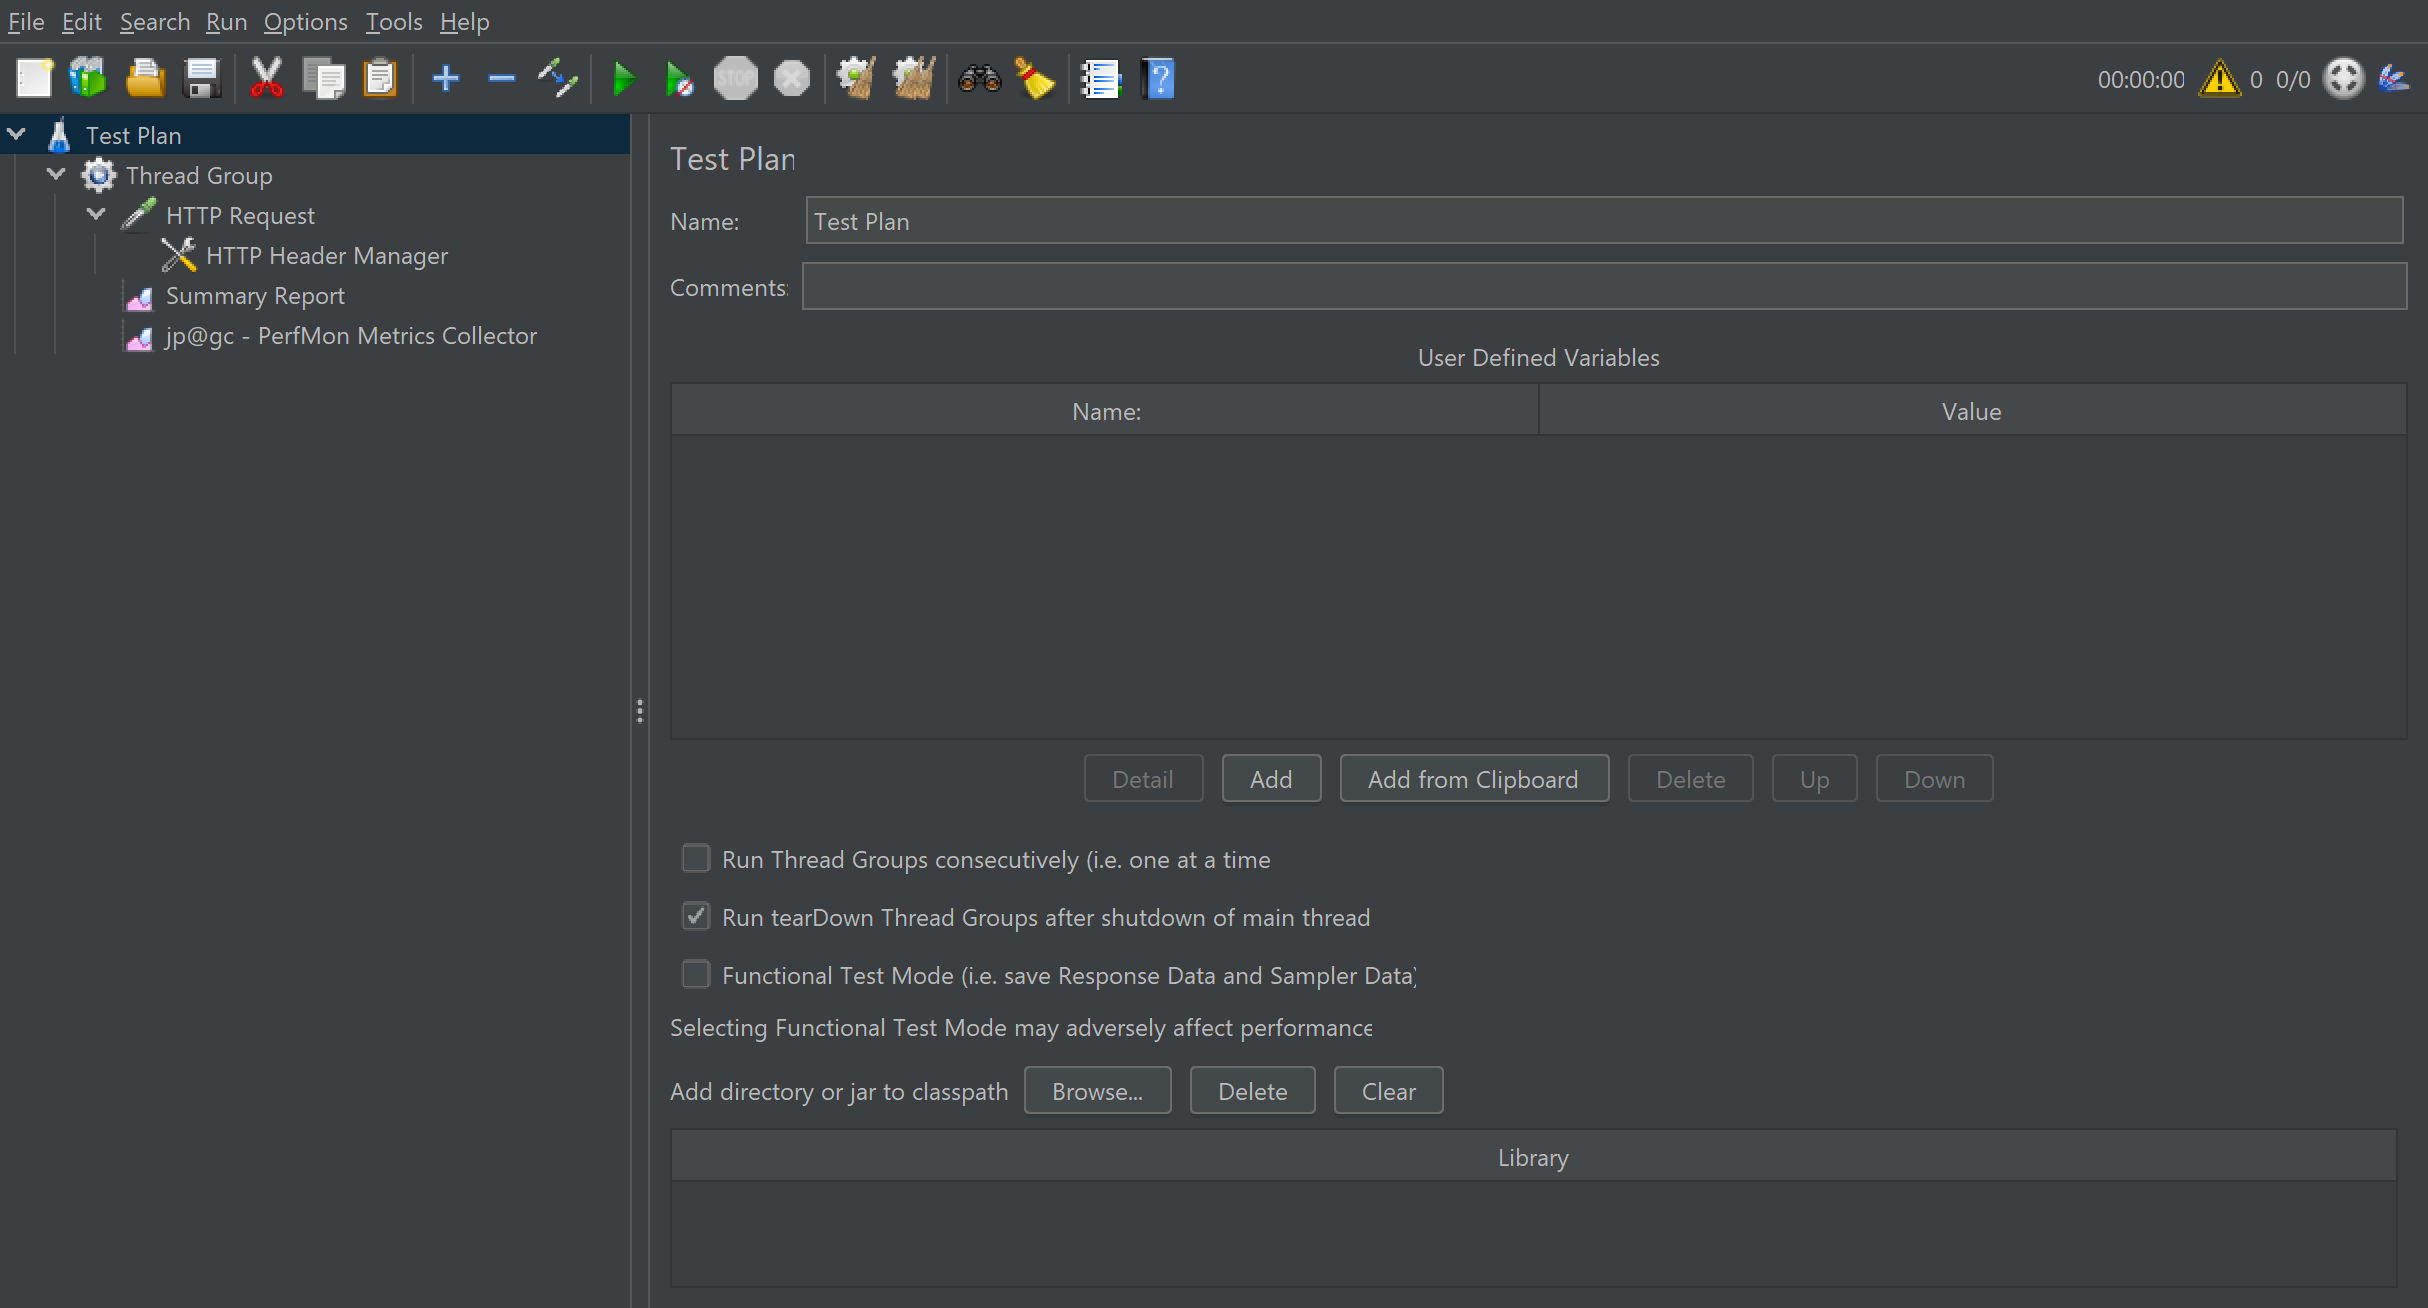
\includegraphics[width=1.0\textwidth]{gfx/Test Plan-Last.png}
  \caption{Test Plan-Last}
  \label{fig:chapter03:TestPlan-Last}
\end{figure}
\bigskip

In \autoref{fig:chapter03:TestPlan-Last} ist eine Gesamtübersicht des Testplans dargestellt. In Thread Group wurde die Konfiguration vorgenommen, die in Abbildung 22 dargestellt ist. Hier wurden zwei Listener konfiguriert, nämlich Summary Report und jp@gc – Performance Metrics Collector. Summary Report ist für das Protokollieren der Messdaten zuständig. Hier werden unter anderem die Latenz, Response Time und Connect Time protokolliert. Der Performance Metrics Collector ist für das Messen von CPU-Auslastung und RAM-Belegung zuständig.
In dem HTTP Header Manager wird der HTTP-Header der HTTP-Anfrage, die jeweils an den Server gesendet werden soll, konfiguriert. 

\begin{figure}[htbp]
  \centering
  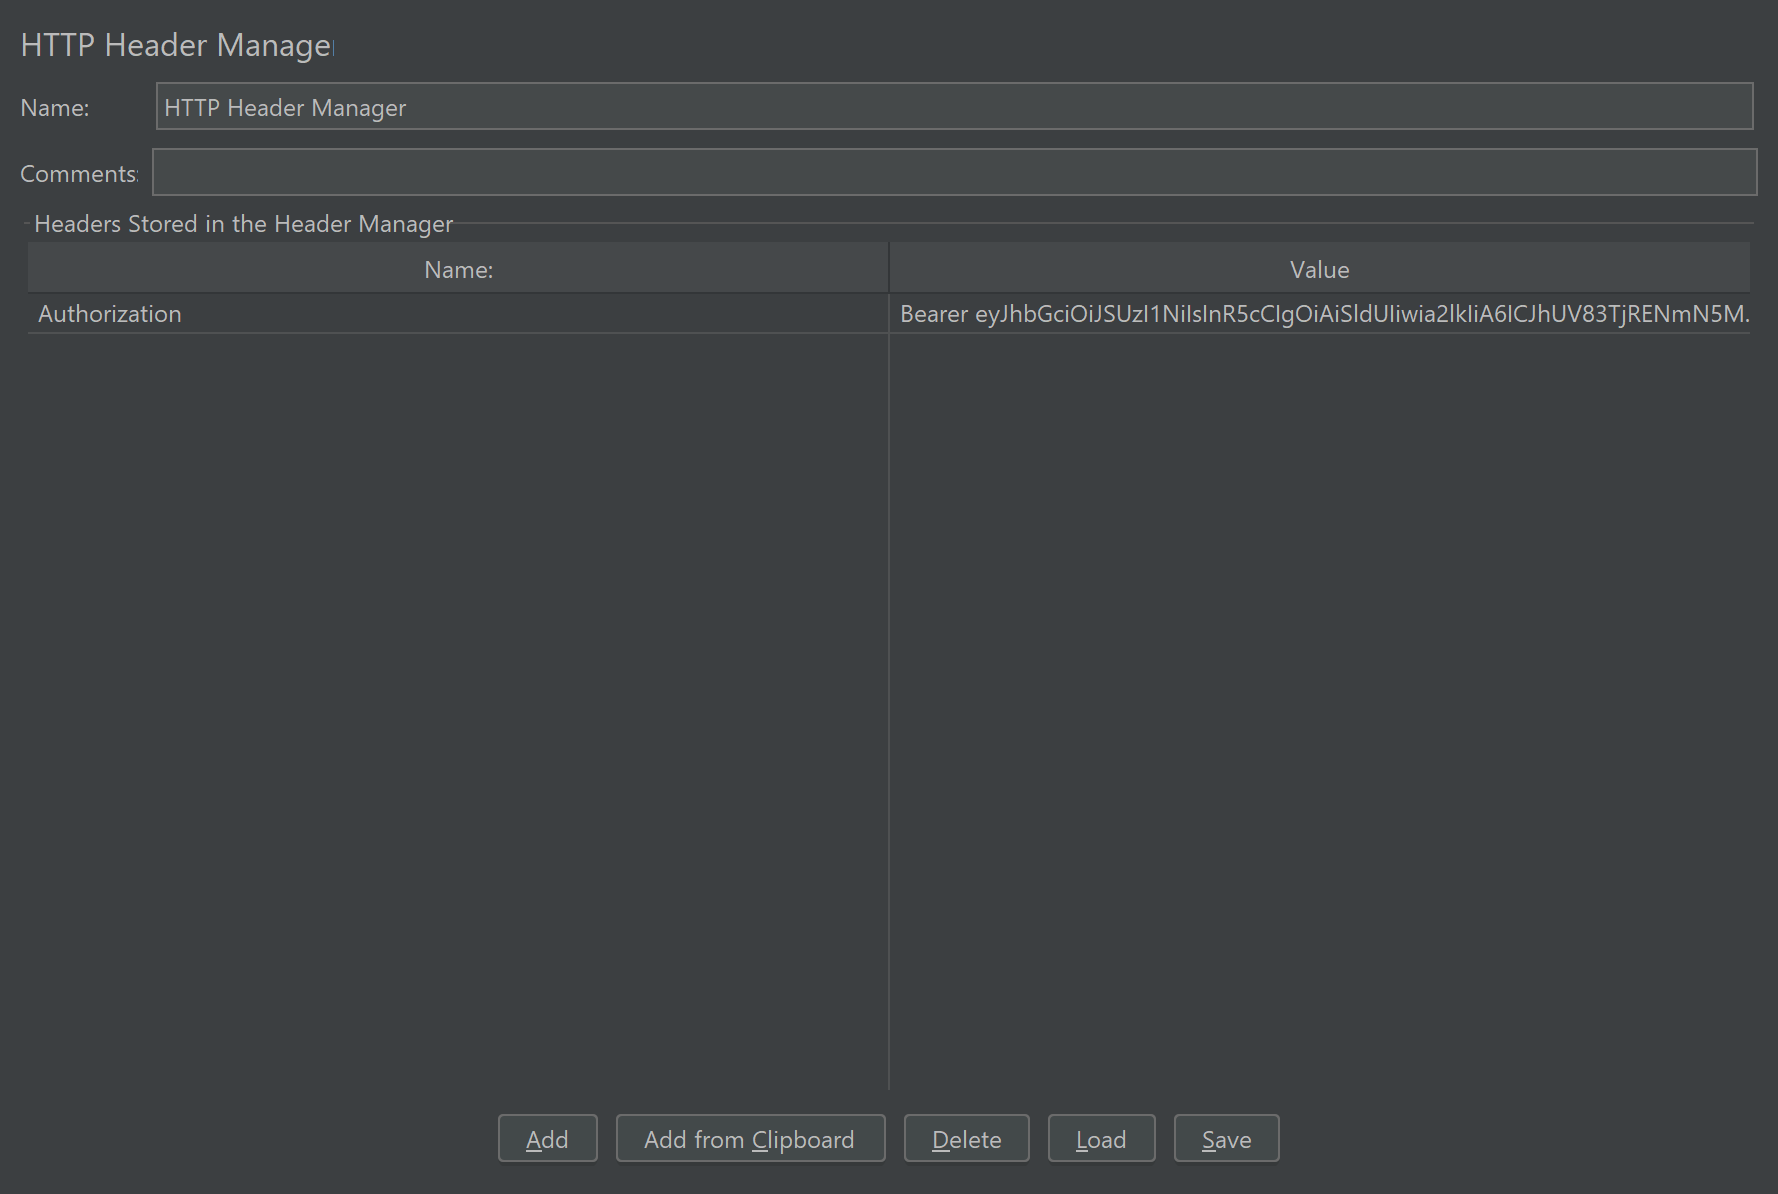
\includegraphics[width=1.0\textwidth]{gfx/HTTP Header Manager.png}
  \caption{HTTP Header Manager}
  \label{fig:chapter03:HTTPHeaderManager}
\end{figure}
\bigskip

In \autoref{fig:chapter03:HTTPHeaderManager} ist der verwendete HTTP Header Manager zu sehen. Hier wurde lediglich der JSON Web Token in dem Schlüssel Authorization des HTTP-Headers hinterlegt. Der Erhalt des Tokens wurde in Kapitel 3.2 beschrieben. Als Prefix wird Bearer angegeben, um dem empfangenden System zu signalisieren, dass in dem Authorization-Feld des HTTP-Headers ein Bearer Token steht, das heißt ein durch OAuth2 erlangter Token [8].

\begin{figure}[htbp]
  \centering
  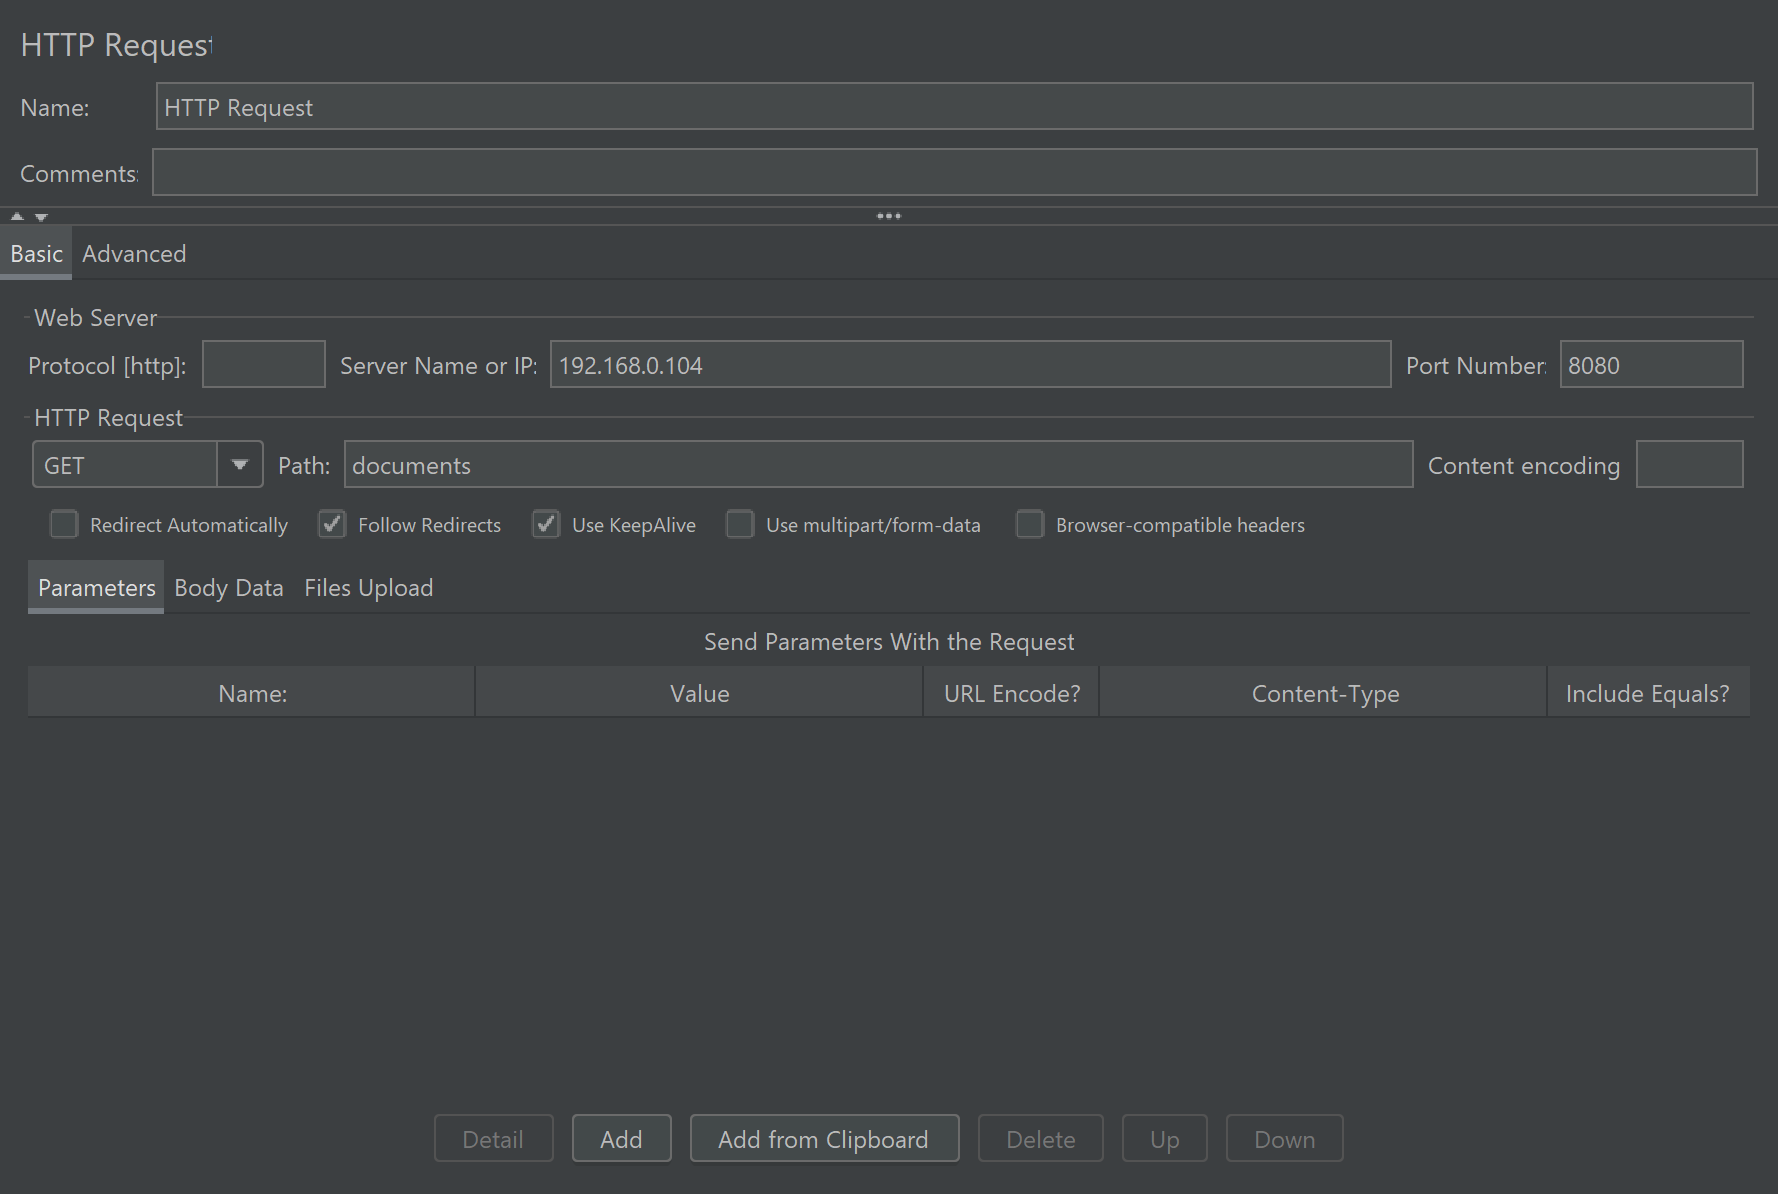
\includegraphics[width=1.0\textwidth]{gfx/HTTP Request.png}
  \caption{HTTP Request}
  \label{fig:chapter03:HTTPRequest}
\end{figure}
\bigskip

In \autoref{fig:chapter03:HTTPRequest} ist die HTTP-Anfrage zu sehen, die jeweils an den Server gesendet wird. Hier wurde die Anfragemethode auf GET eingestellt und der Pfad auf documents gesetzt, denn die Schnittstelle des Ressource Server ist wie in Kapitel 3.3.1 erläutert eine HTTP-GET-Schnittstelle. In dem Feld Server Name or IP wurde die IP-Adresse des Servers angegeben. Bei den Tests wird der Client, Apache JMeter, und Server auf zwei Rechnern gestartet, damit die Testergebnisse nicht verfälscht werden. 

\subsection{Skalierbarkeitstest}
Bei dem Skalierbarkeitstest geht es darum, eine ansteigende Last zu generieren, um herauszufinden inwiefern sich die Latenzen verändern. Je mehr Last erzeugt wird, desto höher werden tendenziell die Latenzen. 

\begin{figure}[htbp]
  \centering
  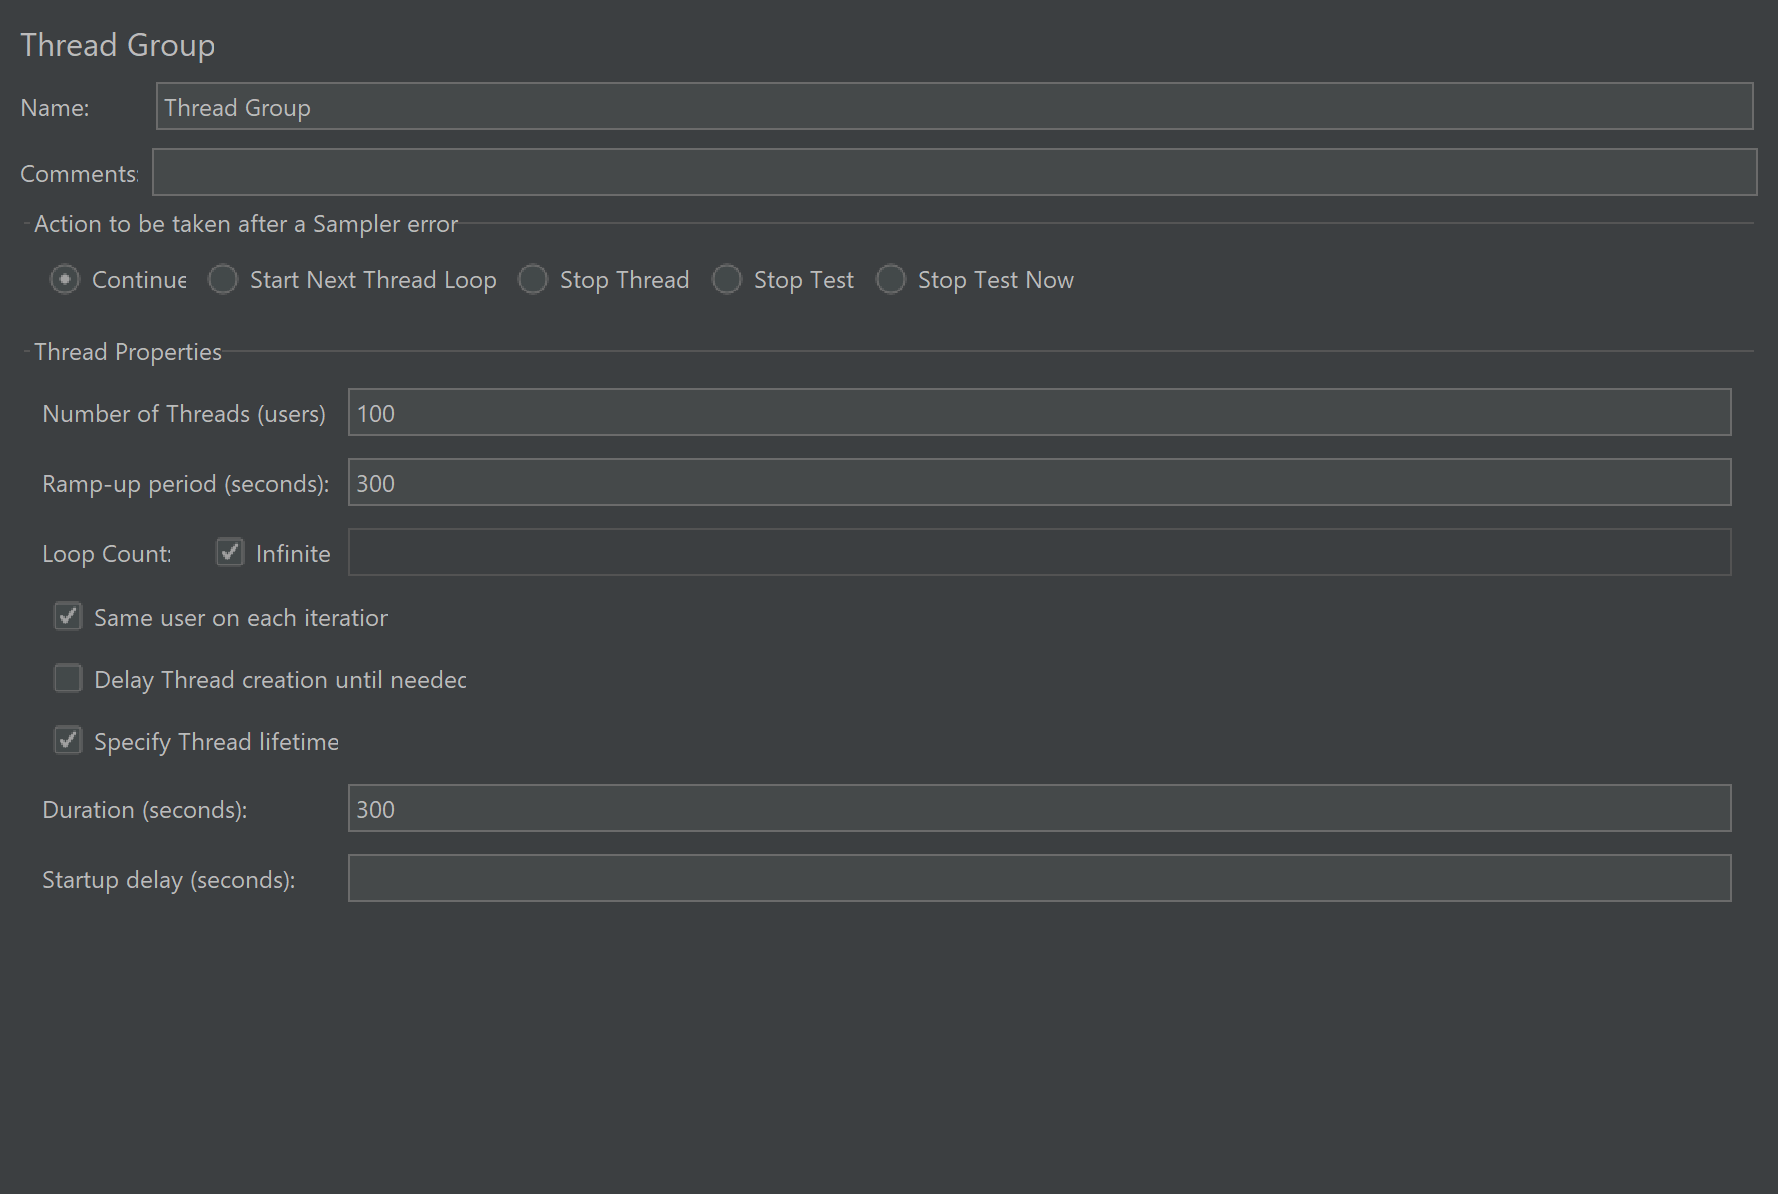
\includegraphics[width=1.0\textwidth]{gfx/Thread Group-Skalierung.png}
  \caption{Thread Group-Skalierung}
  \label{fig:chapter03:ThreadGroup-Skalierung}
\end{figure}
\bigskip

In \autoref{fig:chapter03:ThreadGroup-Skalierung} ist die verwendete Konfiguration zu sehen. Es werden 100 Threads gestartet, wobei hier die Ramp-up period 300 beträgt, dass bedeutet das erst nach 300 Sekunden alle 100 Threads gestartet wurden. Es werden pro Sekunde 300/100 = 3 Threads gestartet. Die Gesamtdauer des Tests beträgt 300 Sekunden, das heißt 15 Minuten. 
Was dadurch ermöglicht wird, ist das bis zum Ende des Tests eine ansteigende Last auf den Server entsteht. Dadurch lässt sich betrachten, inwiefern sich die Latenzen beziehungsweise Response Times der Anfragen bei ansteigender Last verhalten. 

\subsection{Stresstest}
Das Ziel des Stresstests ist es, eine möglichst hohe Last auf den Server zu erzeugen, um die Grenzen des Systems auszuloten. Es ist wichtig zu wissen, wie viele Nutzer ein System gleichzeitig bedienen kann, bis das System entweder unerreichbar wird oder die Latenzen der Antworten unakzeptabel hoch sind, damit dem zum geeigneten Zeitpunkt durch horizontale Skalierung entgegengewirkt werden kann. Zudem können durch diesen Test, Schwachstellen der jeweiligen Implementierungen wie beispielsweise Memory Leaks, erkannt werden. 

\begin{figure}[htbp]
  \centering
  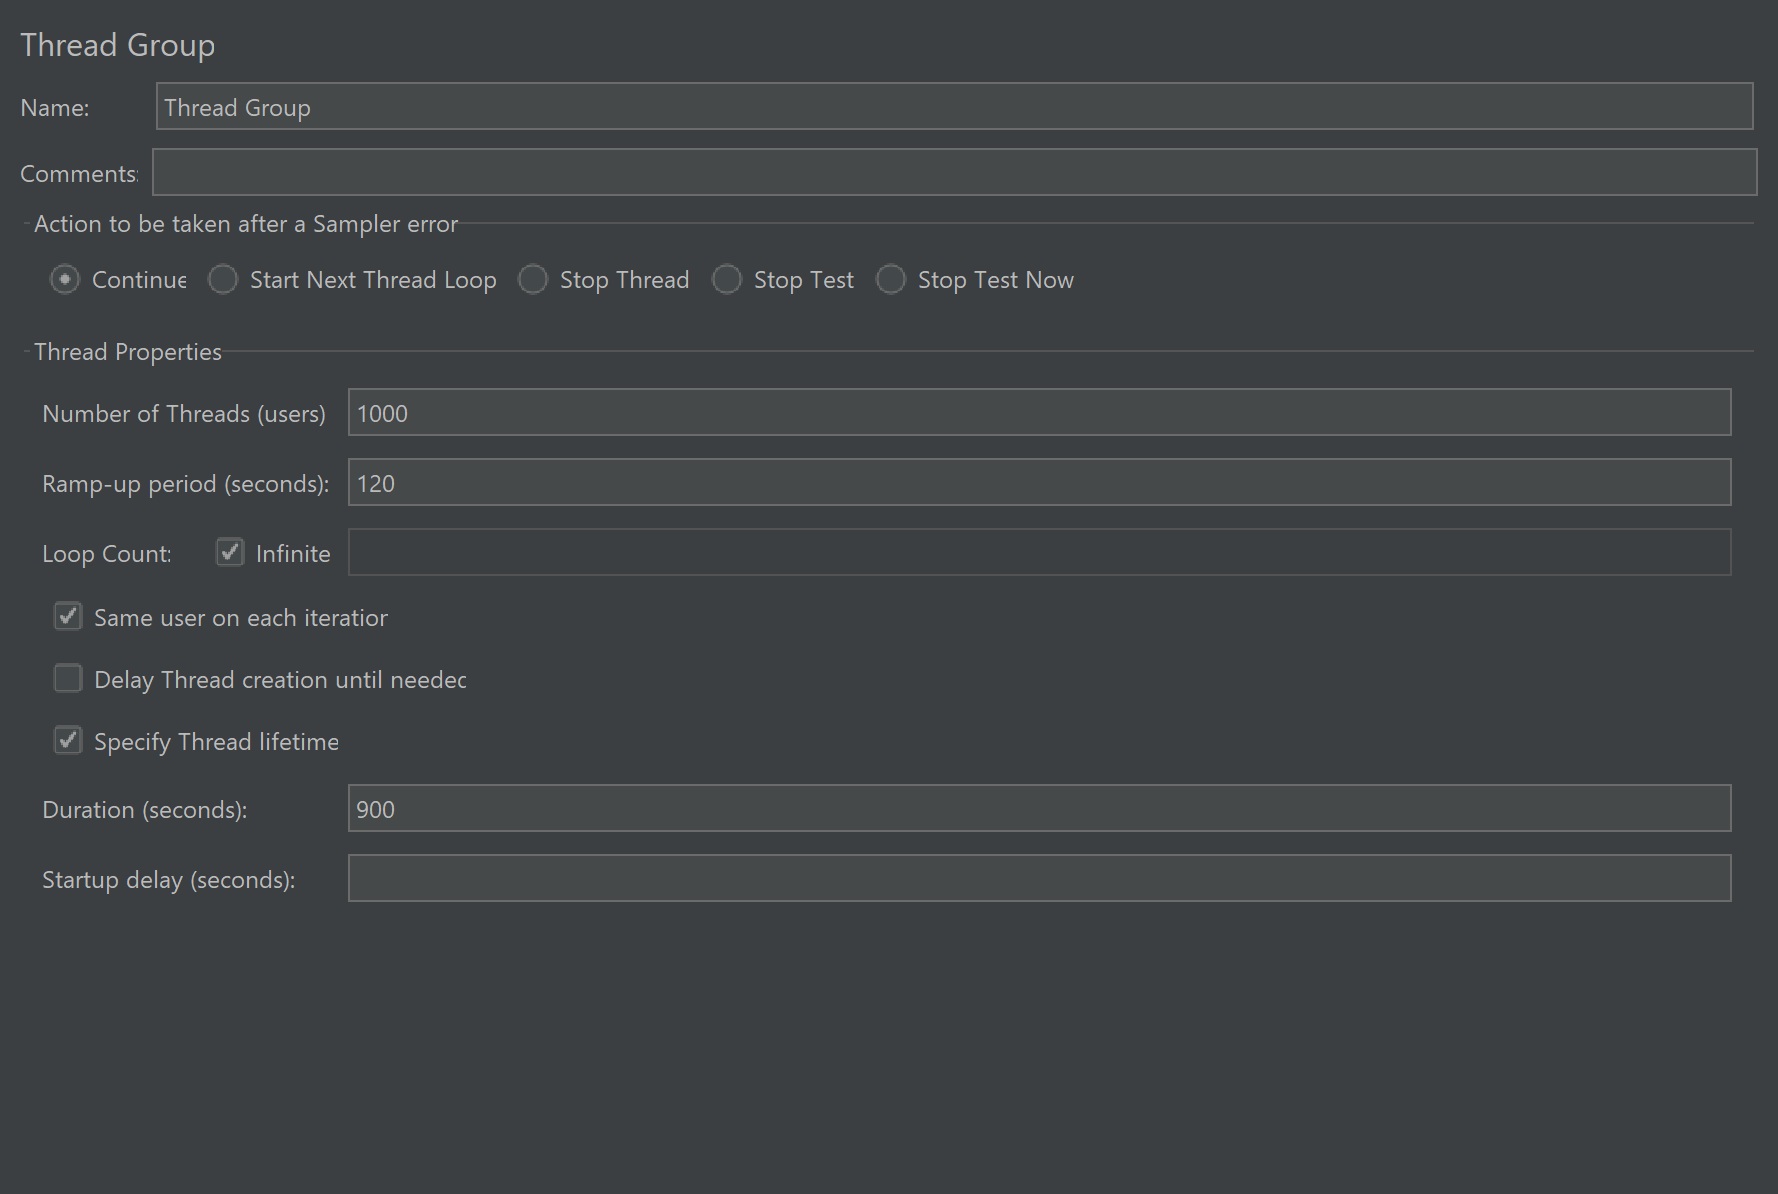
\includegraphics[width=1.0\textwidth]{gfx/Thread Group-Stress.png}
  \caption{Thread Group-Stress}
  \label{fig:chapter03:ThreadGroup-Stress}
\end{figure}
\bigskip

In \autoref{fig:chapter03:ThreadGroup-Stress} ist die verwendete Konfiguration zu sehen. Es werden insgesamt 1000 Threads gestartet wobei alle 1000 Threads erst nach 120 Sekunden gestartet sind. Der Test dauert insgesamt 900 Sekunden, das heißt 15 Minuten. Während dieser Zeit sendet jeder Thread kontinuierlich Anfragen an den Server. Dieser Test ist deutlich ressourcenintensiver als der Last-und-Skalierbarkeitstest. Verlässlich können pro Maschine in Apache JMeter, ca. 1000-2000 Threads gestartet werden, was allerdings abhängig ist von der jeweiligen Hardware des Systems, auf dem Apache JMeter ausgeführt wird \citep{jmetermaxthreads:2017}. Dieser Test wird ohne die GUI von Apache JMeter ausgeführt, da diese speziell bei ressourcenintensiven Stresstests die Testergebnisse verfälschen kann. Die verwendete Systemhardware von Client und Server werden im Kapitel Systemhardware beschrieben. 

\subsection{Messung und Protokollierung von Messdaten}
Um die Messdaten der Tests aus den vorrangegangenen Kapiteln zu protokollieren und in geeigneter Weise zu visualisieren, wurden Apache JMeter Listener verwendet, die Messdaten in Comma-separated values (CSV)-Dateien schreiben. Um diese Daten visuell darzustellen, wurde der HTML Report von Apache JMeter verwendet. Als Listener wurde jeweils Summary Report verwendet. Dieser misst und protokolliert unter anderem die folgenden Daten: 
\begin{itemize}
  \item Response Time
  \item HTTP-Status Code der Antwort des Servers
  \item Latenz
  \item Connect Time
  \item Gesendete Bytes
  \item Erhaltene Bytes
\end{itemize}
\smallskip

Für die Bestimmung des Application Performance Index wurden folgende Werte gewählt:

\begin{table}[h]
  \myfloatalign
  \begin{tabularx}{\textwidth}{|l|l|X|} \toprule
      \tableheadline{Level} & \tableheadline{Multiplier} & \tableheadline{Time T} \\ \midrule
      Zufrieden & <= T & <= 500 Millisekunden  \\
      \midrule
      Toleriert & >T, <= 3T & [0,5 Sekunden, 1,5 Sekunden]  \\
      \midrule
      Frustriert & > 3T & > 1,5 Sekunden  \\
      \bottomrule
  \end{tabularx}
  \caption[Application Performance Index]{Application Performance Index.}
  \label{tab:ApplicationPerformanceIndex2}
\end{table}

Das bedeutet, dass Nutzer bis zu einer Response Time von 500 Millisekunden zufrieden sind. Response Times bis 1500 Millisekunden tolerieren Nutzer und bei Response Times ab 1500 Millisekunden sind Nutzer frustriert. Der Multiplier ist hier 3T. Aus diesen Werten wird der Performance Index berechnet.

\section{Systemhardware und Testumfeld}
\label{subsec:SystemhardwareundTestumfeld}
Es wird die verwendete Systemhardware für Client und Server, die in allen drei Tests verwendet wurde, aufgelistet. Dies ist erwähnenswert, da die Messwerte von der Leistungsfähigkeit der Hardware abhängen. Da allerdings ein Vergleich zwischen zwei Systemen gezogen wird, können auch allgemeingültige Erkenntnisse aus den Ergebnissen der Tests gezogen werden. Ein weiterer wichtige Punkt ist der, dass beide Rechner, Client und Server, sich in demselben Netzwerk befinden und über denselben Router über Ethernet mit dem Internet verbunden sind. 
Open Policy Agent wird in einem Docker-Container ausgeführt und für die Simulierung der virtuellen Maschine des Docker-Containers wird \ac{WSL 2} verwendet. Für die Ressourcenbereitstellung des Docker-Containers, wurden die Standardeinstellungen verwendet. Diese sind in der Dokumentation von Microsoft vorzufinden \citep{wsl:2021}. Das bedeutet, der Docker-Container kann alle Prozessorkerne verwenden und ist bei der Arbeitsspeicherbelegung auf 8 Gigabyte begrenzt. 

\begin{table}[h]
  \myfloatalign
  \begin{tabularx}{\textwidth}{|l|X|} \toprule
      \tableheadline{Komponente} & \tableheadline{Spezifikation} \\ \midrule
      CPU & Intel(R) Core(TM) i5-8265U CPU @ 1.60GHz \\
      \midrule
      Arbeitsspeicher & 16 Gigabyte \\
      \midrule
      Betriebssystem & Microsoft Windows 10 Pro, 64 Bit Version	10.0.19042 Build 19042 \\
      \bottomrule
  \end{tabularx}
  \caption[System des Clients]{System des Clients.}
  \label{tab:SystemdesClients}
\end{table}

In \autoref{tab:SystemdesClients} ist das System des Clients dargestellt. Auf diesem System wird Apache JMeter ausgeführt, es sendet jeweils die HTTP-Anfragen an den Server. 

\begin{table}[h]
  \myfloatalign
  \begin{tabularx}{\textwidth}{|l|X|} \toprule
      \tableheadline{Komponente} & \tableheadline{Spezifikation} \\ \midrule
      CPU & Intel(R) Core(TM) i7-7700HQ CPU @ 2.80GHz \\
      \midrule
      Arbeitsspeicher & 16 Gigabyte \\
      \midrule
      Betriebssystem & Microsoft Windows 10 Education, 64 Bit Version	10.0.19042 Build 19042 \\
      \bottomrule
  \end{tabularx}
  \caption[System des Servers]{System des Servers.}
  \label{tab:SystemdesServers}
\end{table}

In \autoref{tab:SystemdesServers} ist das System des Servers dargestellt. Hier laufen die jeweiligen Ressource Server, die die Anfragen von Apache JMeter beantworten.